\chapter{The KamLAND-ZEN Experiment}
\label{chapter:klz-detector}
\thispagestyle{myheadings}
\graphicspath{{2_Chapter_KLZ_Detector/Figures/}}

KamLAND, the \textbf{Kam}ioka \textbf{L}iquid-scintillator \textbf{A}nti Neutrino \textbf{D}etector, is a large liquid scintillator calorimeter detector situated 1km below mt. Ikenoyama in Gifu prefecture, Japan. I will describe the KamLAND detector's and the corresponding KamLAND experimental area's important components and features in this chapter. I will also explain how each component contributes to the KamLAND's scientific goals and the work of this thesis.


\section{KamLAND}
\label{sec:KamLAND}
One can think of KamLAND as an onion made up of many spherical layers, each layer serving the ultimate goal of shielding and observing the central core, the xenon-loaded liquid scintillator.


\subsection{Detector Infrastructure and Outer Detector}
The KamLAND detector is surrounded by the KamLAND experimental area, situated in an old iron mine, multiple caverns and passageways were excavated and set aside for KamLAND experimental use.

The KamLAND site is shown in Figure *. The control room contains networking and monitoring equipment which on-site shifters use to observe real-time detector activity. The first LS purification areas contain liquid-liquid extraction and nitrogen purge purification systems. The second LS purification area contains a distillation purification system. A new Xenon purification area was built for KamLAND-Zen. The dome area is a class 1,000 clean area atop the detector and includes a calibration source preparation room and electronics enclosure (electronics hut or e-hut). At the center of the dome area, there is a secondary class 100-1000 clean tent covering the KamLAND chimney. The inner balloon installations took place in August 2016 and May 2018 inside this clean tent.

The outer detector (OD) is a cylindrical water tank 20m tall and with 20m diameter and filled with pure water. The OD was refurbished in 2016, and 140 new 20-inch PMTs (R3600) were installed inside the cavity. The inner wall of the outer tank and the outer surface of the inner detector stainless steel spherical tank are covered highly reflective Tyvek sheets (Tyvek 1073B and 1082D) to collect as much of the light generated by crossing cosmic ray muons as possible. The outer detector's role is to tag cosmic ray muons, shield radioactivity and fast neutrons from the outer rock, and to stabilize the temperature of the ID.

\subsection{Inner Detector}
KamLAND's inner detector (ID) is the main spherical liquid scintillator detector, it is shown in Figure *. The ID is contained in a 18m diameter stainless steel sphere tank. 1,879 PMTs are mounted onto the inner wall of the ID, 1,325 17-inch and 554 20-inch PMTs. The PMTs are submerged in non-scintillating buffer oil (BO). An acrylic panel separates the buffer layer into two shells. This panel prevents the convection of radon out-gassed from PMT glasses into the central parts of the detector.

Photomultiplier tubes (PMTs) are KamLAND's eyes, detecting individual photons of light emitted by passage of particles through the scintillator volumes. Photons that hit PMT photocathodes are converted into a photoelectron. This photoelectron is then guided by electric fields to a series of dynodes. Each dynode multiplies the photoelectrons many times over, until the first photoelectron becomes $10^{6-7}$ electrons. Should multiple photons hit the photocathode simultaneously, the output voltage increases proportionally. This current is converted to a voltage by a coupling capacitor and read out via long coaxial cables. Figure ~\ref{fig:pmts} is a diagram of the 17in and 20in PMTs.

The 1,325 17-inch PMTs are Hamamatsu R7250s while the 554 20-inch PMTs are Hamamatsu R1449s and R3600s. The 20-inch PMTs were inherited from the Kamiokande experiment to increase our light collection. Both sets of PMTs have a bialkali photocathode sensitive to 300-650nm light which is well-suited for the emission spectrum of the LS. Figure ~\ref{fig:pmtqe} shows the quantum efficiency of the PMTs. The pmts also differ by dynode design; while the 17-inch PMTs feature "box-and-line" designs, the 20-inch PMTs have "venetian-blind styles". The different dynode designs along with the masking on the 17-inch PMTs, give us 17-in PMTs with better transit time spread (TTS) and 20-inch PMTs with better light collection efficiency. In total, the photocathode coverage of the ID is 34\%, with 23\% contributed by the 17-inch PMTs.

Furthermore, the PMT performance can be affected by the earth's magnetic field. To reduce this unwanted effect, the entire KamLAND detector is surrounded by geomagnetic compensation coils to counteract this external magnetic field. The residual magnetic field is less than 50mG, which has negligible effect on the PMT performance.

Another important characteristic of PMTs is their quantum efficiency (QE). The QE quantifies the probability that a photon arriving on the photocathode will produce a photoelectron. A PMT's QE varies over the wavelength of the incoming light. To improve our light collection, KamLAND's LS is doped with PPO to shift the wavelength of the incoming light to where the PMTs are most sensitive. Figure ~\ref{fig:qe_ppo} shows the PMT QE curve and the PPO reemission spectrum.

Next, is the 13m diameter outer balloon (OB). The OB is suspended in the center of the ID within the buffer oil, it is filled with one kiloton of highly purified organic liquid scintillator.

\subsection{Liquid Scintillator}
Liquid scintillator (LS) is the vital medium that sensitizes KamLAND to internal radioactivity. The KamLAND LS (KamLS), found in between the outer balloon and inner balloon, is composed of 80.2\% of dodecane (D12),1,2,4-trimethyl benzene, and 19.8\% pseudocumene (PC). A wavelength shifter called 2,5-diphenyloxazole (PPO) is added to the LS at a concentration of $1.36 \pm 0.03$ g/L. KamLAND-Zen has achieved $5 \times 10^{-18}$ g/g and $1.3 \times 10^{-17}$ g/g contamination for 238U and 232Th, respectively. The chemical composition of the KamLS can be found in Table ~\ref{tbl:kamls}

\begin{table}[h]
	\centering
	\renewcommand{\arraystretch}{1.2}
	\begin{tabular}{c|ccc}
		\hline
		& D12 & PC & PPO \\
		\hline
		Chemical Formula & C$_{12}$H$_{26}$ & C$_9$H$_{12}$ & C$_{15}$H$_{11}$NO \\
		Density [$g/cm^3$] & 0.7526 & 0.8796 & -\\
		Boiling Point [$^\circ$C] & 216 & 169 & 360 \\
		Melting Point [$^\circ$C] & -10 & -44 & 72 \\
		Flash Point [$^\circ$C] & 83 & 54 & - \\ \hline
	\end{tabular}
	\caption{Composition and properties of KamLAND Liquid Scintillator (KamLS)}
	\label{tbl:kamls}
\end{table}

\subsection{KamLAND-ZEN and XeLS}
At the center of KamLAND-ZEN lies the Xenon-loaded Liquid Scintillator (XeLS) contained in the 1.9m radius inner balloon (IB). The double-beta decaying isotope $^{136}Xe$ is thus placed in the cleanest, most sensitive part of the experiment. The Xenon gas is enriched to 90\% $^{136}Xe$ and is dissolved into a modified version of KamLS. The PPO concentration was increased to 4g/L to boost the light yield. This increased PPO concentration compensates for the 10\% reduction in emitted scintillation light when Xenon is mixed into the LS. The XeLS density is also tuned to match the surrounding KamLS. The chemical composition of the XeLS is shown in Table \ref{tbl:xels} in each of the different phases of the KamLAND-ZEN experiment.

\begin{table}[h]
	\centering
	\renewcommand{\arraystretch}{1.2}
	\begin{tabular}{c|cccc}
		\hline
		Material & Decane (\%) & PC (\%) & PPO (\%) & Xe (\%)\\ \hline
		Zen 400 Phase-1 & 82.3 & 17.7 & 2.7 & 2.44/2.48\\
		Zen 400 Phase-2 & 80.7 & 19.3 & 2.29$\pm$0.03 & 2.91\\
		Zen 800 & 82.4 & 17.6 & 2.38$\pm$0.02 & 3.13\\ \hline
	\end{tabular}
\end{table}

\section{Chemical Handling Infrastructure}
Background mitigation is crucial for \0nbb. Maintaining the purity of the liquid volumes inside KamLAND is an important part of background mitigation in KamLAND-ZEN. In this section, we will briefly describe the systems that provided or maintain the purity of the LS and XeLS in KamLAND.

\subsection{Water Extraction}
The first purification is shown in Figure ~\ref{fig:waterex}. Both the liquid scintillator and buffer oil are filtered in two stages with 1$\mu$m and 0.1$\mu$m pore sizes respectively. Next, the liquids are flushed with pure water in the water extraction tower where metals such as U, Th, and K, are absorbed by the water. Finally, the liquids are purged with ultra-pure nitrogen gas to remove gaseous contaminants like radon and oxygen.

\subsection{Distillation}
The next purification system utilizes the distillation system shown in Figure ~\ref{fig:distillation}. LS from KamLAND is constantly cycled through the distillation system. There boiling is done to separate the individual chemical components of KamLS, namely Pseudocumene (PC) and PPO. Each component is individually distilled and purified. Then, the components are combined in the mixing tank to the original LS composition with an accuracy of $10^{-3}g/cm^3$. Finally high-purity nitrogen gas is used to purge the LS coming out of the mixing tank to eliminate any gaseous contaminants.

\subsection{Xenon Handling}
A schematic diagram of the XeLS handling system is shown in Figure~\ref{fig:xenonhandling}. The system consists of the following components:
\begin{itemize}
	\item A \textbf{1.1 m$^3$ Main Tank} directly connected to KamLAND-ZEN's inner balloon. The extracted XeLS first enters this tank.
\end{itemize}

\begin{figure}[htb]
	\centering
	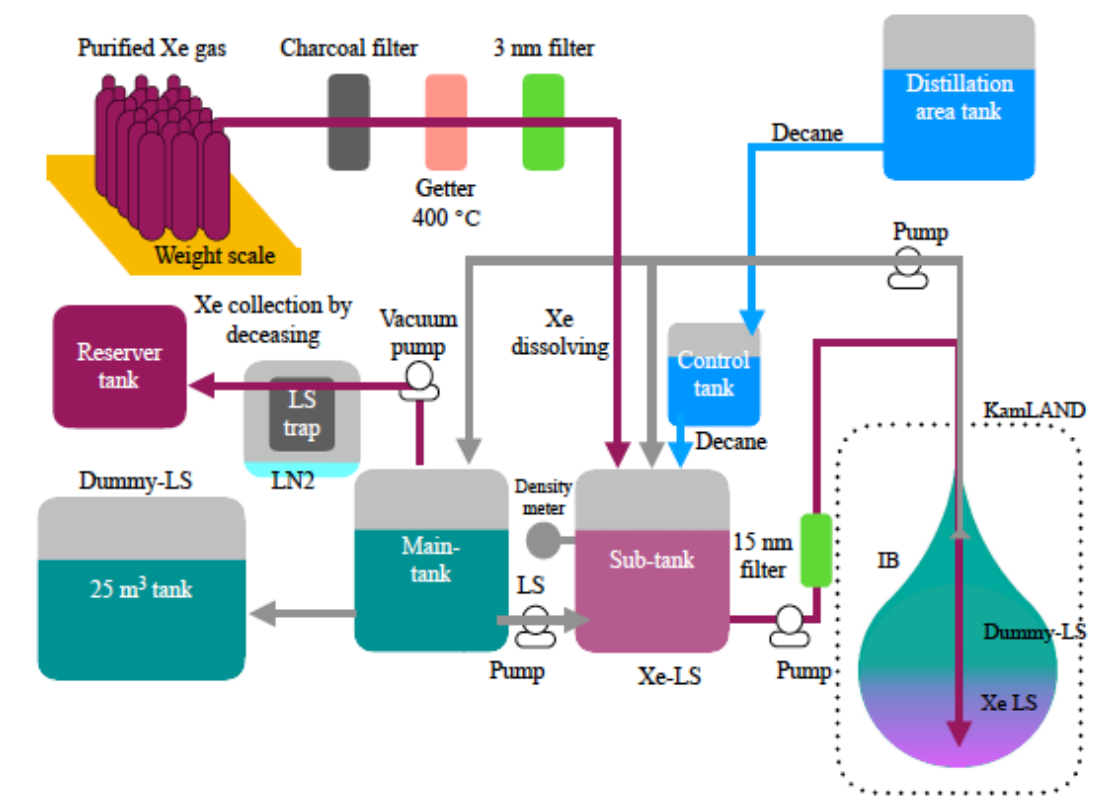
\includegraphics[scale=0.5]{xenonhandling.png}
	\caption{Flow diagram of the KLZ Xenon system. The purple lines denote the flow of Xe/XeLS, the blue line denotes the flow of decane, the the grey line denotes the flow of LS. Figure from Reference }
	\label{fig:xenonhandling}
\end{figure}

\section{Data Acquisition}

\section{KamLAND-ZEN Phases}

\subsection{KamLAND-ZEN 400}

\subsection{KamLAND-ZEN 800}

% Of course, there must be a Table of Contents, List of Figures and List of Tables at the beginning of the thesis, but this is all set up automatically.

{\bf Important}: You will also be using a lot of citations. The format in this template follows the so-called APA style and looks as follows in the document body: \cite{lamport1985:latex}, \cite{Debr01}. There are no numbers in the list of references -- the list is sorted alphabetically according to the first author's last name.

% Other styles of references are allowed by the library as well, e.g., ``plain'' or ``'ieee'', which use numbers in square brackets both in the document body and in the list of references. In order to use another style of references, e.g., ``plain'', follow the steps below:
% %
% \begin{enumerate}
%   \item In ``thesis.tex'' file:
% 	\begin{itemize}
% 	  \item comment out the line ``$\backslash$usepackage\{apalike\}'' at the top of the file,
% 	  \item replace ``$\backslash$bibliographystyle\{apalike\}'' with ``$\backslash$bibliographystyle\{plain\}'' towards the bottom of the file.
% 	\end{itemize}
%   \item In ``bu\_ece\_thesis.tex'' file, comment out all lines in the BIBLIOGRPAHY section (lines 503-517) and save it!
%   \item Recompile ``thesis.tex'' twice
% \end{enumerate}

